\chapter{第三部分}
\section{问题概述}
%
%%对问题的直观描述
%
该部分包含第7、8小题。

该部分所要解决的问题是帮助吃豆人收集迷宫中所有的食物,食物个数和位置不定。题目要求为该问题设计一个一致的启发式函数。
同时,题目要求实现findPathToClosetDot函数并补充完整AnyFoodSearchProblem类的目标检测函数,帮助吃豆人找到前往最近食物的路径,以找到上述问题的一个近似最优解。
%
%对项目已有代码的阅读和理解
%

%
%解决问题的思路和想法
%

\section{算法设计}
%
%用自己的语言描述解决问题所使用的算法的原理及功能,设计思路和算法流程图
%
一开始我尝试使用最小生成树的总代价作为启发式函数,但是经过测试后发现这并不一致。后来我尝试使用当前位置到各个目标位置的曼哈顿距离的最大值作为启发式函数,
但是需要展开的结点过多,只能获得部分分数。受此启发,我在此基础上进一步优化,将启发式函数调整为各个目标位置加上当前位置所组成的集合中,任意两个位置之间的曼哈顿距离的最大值,
这一启发式函数能够得到附加分之外的所有分数。

由于吃豆人移动一格时,上述集合中的任意两个元素之间的曼哈顿距离最多减少一个单位,因此最大值最多减少一个单位,即由此定义的启发式函数最多减少一个单位,即该启发式函是一致的。

对于AnyFoodSearchProblem类,它的目标是收集到任意一个食物。因此它的目标检测函数只需判断当前位置是否属于由目标位置组成的集合即可。

在已给的代码中,findPathToCloseDot函数中创建了一个AnyFoodSearchProblem的实例,这提示我们利用该问题来辅助完成该函数的实现。这里所要求的前往最近食物的路径实际上就是
AnyFoodSearchProblem的一个深度最浅的解。因此只需要使用BFS求解该问题即可。
\section{算法实现}
%
%在算法原理的基础上,结合代码,讲述算法的实现细节、和兴函数、模块输入输出,数据结构定义等内容
%
\begin{lstlisting}[emph={[3]parent,pathCost,problem,heuristic,state,goals,position},emphstyle={[3]\color{vscode_parametercolor}},emph={[4]SearchProblem,Callable,Node,Reached,Any,Tuple,List,FoodSearchProblem},emphstyle={[4]\color{vscode_classcolor}}]
def foodHeuristic(state: Tuple[Tuple, List[List]], problem: FoodSearchProblem):
    position, foodGrid = state
    nodes = foodGrid.asList()
    nodes.append(position)
    distance = [manhattanDistance(nodes[i], nodes[j]) for i in range(len(nodes) - 1) for j in range(i + 1, len(nodes))]
    return max(distance) if distance else 0  # 确保目标结点的启发式函数值为0
\end{lstlisting}
下面给出的是AnyFoodSearchProblem类的目标检验函数的实现:
\begin{lstlisting}[emph={[3]parent,pathCost,problem,heuristic,state,goals,position},emphstyle={[3]\color{vscode_parametercolor}},emph={[4]SearchProblem,Callable,Node,Reached,Any,Tuple,List,FoodSearchProblem},emphstyle={[4]\color{vscode_classcolor}}]
def isGoalState(self, state: Tuple[int, int]):
    x, y = state
    return self.food[x][y]
\end{lstlisting}
下面给出的是findPathToClosestDot的实现:
\begin{lstlisting}[emph={[3]parent,pathCost,problem,heuristic,state,goals,position,gameState},emphstyle={[3]\color{vscode_parametercolor}},emph={[4]SearchProblem,Callable,Node,Reached,Any,Tuple,List,FoodSearchProblem,pacman,GameState},emphstyle={[4]\color{vscode_classcolor}}]
def findPathToClosestDot(self, gameState: pacman.GameState):
    startPosition = gameState.getPacmanPosition()
    food = gameState.getFood()
    walls = gameState.getWalls()
    problem = AnyFoodSearchProblem(gameState)
    return breadthFirstSearch(problem)
\end{lstlisting}
\section{实验结果}
\subsection{Question7}
成功通过本问题的除了附加测试外的全部测试,实验结果截图见图\ref{q7}。该问题的测试样例,除了最后一个,均为规模较小的迷宫,主要目的是通过各类情况完整地测试设计的启发式函数是否一致。本题附加测试所用的迷宫虽然规模不大,但是它的
食物摆放位置使得我所设计的启发式函数失去了作用——无法正确反映出迷宫中间的墙壁,从而导致$A^*$算法退化,展开的结点较多。

\begin{figure}[htbp]
    \centering
    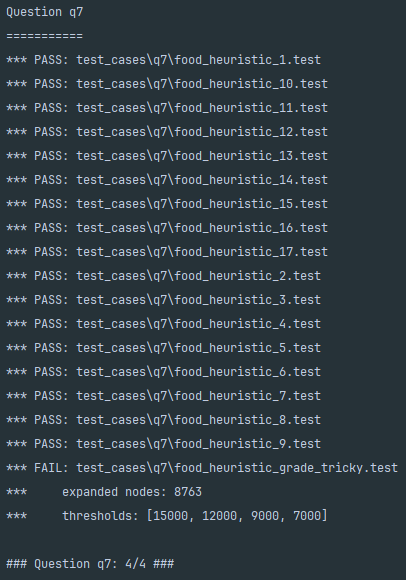
\includegraphics[scale = 0.7]{pic/q7.png}
    \caption{Question7实验结果}\label{q7}
\end{figure}

\begin{figure}[htbp]
    \centering
    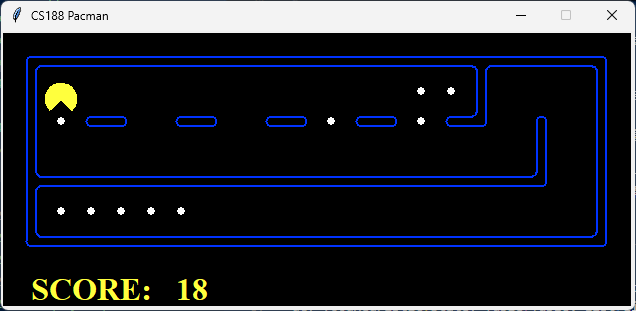
\includegraphics[scale = 0.7]{pic/q7t.png}
    \caption{Question7附加测试}\label{q7t}
\end{figure}
\subsection{Question8}
成功通过本问题的全部测试,实验结果截图见图\ref{q8}。该问题的测试样例均为规模较小的迷宫,用于测试findPathToClosestDot返回的最小路径值是否正确。
\begin{figure}[!htbp]
    \centering
    \begin{minipage}[t]{0.4\textwidth}
    \centering
    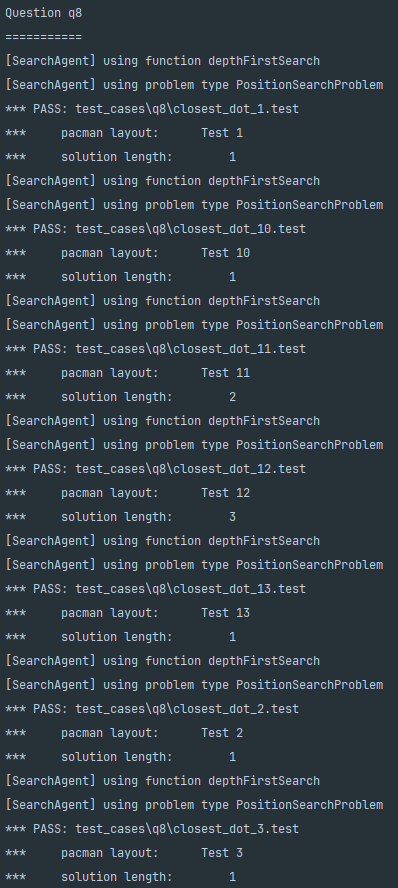
\includegraphics[width=\textwidth]{pic/q81.png}
    \end{minipage}
    \begin{minipage}[t]{0.4\textwidth}
    \centering
    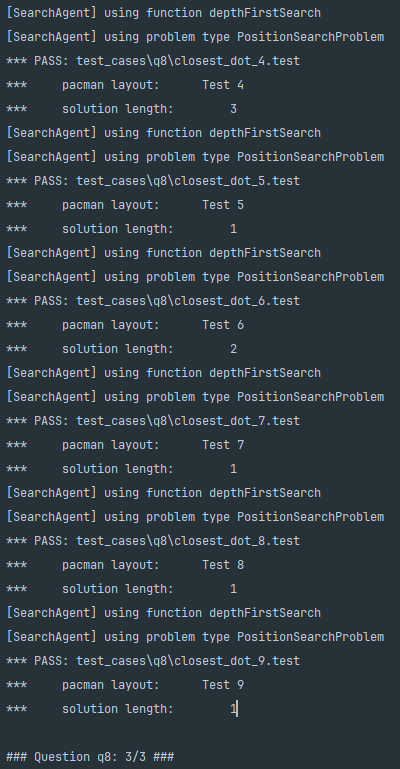
\includegraphics[width=\textwidth]{pic/q82.png}
    \end{minipage}
    \caption{Question8实验结果}\label{q8}
\end{figure}
%
%对试验结果进行详细展示,对每个问题展示测试截图,对于测试用例进行描述说明,对于为通过测试的用例结合自己的算法进行分析,可以结合调试过程进行分析
%
%
%实验中遇到的问题及解决方案,收获和思考:对算法的理解、优缺点的评价、算法的适用场景
%
